
%(BEGIN_QUESTION)
% Copyright 2008, Tony R. Kuphaldt, released under the Creative Commons Attribution License (v 1.0)
% This means you may do almost anything with this work of mine, so long as you give me proper credit

Examine these two variable-resistance ({\it rheostat}) networks, each one with a large-range potentiometer and a small-range potentiometer:

$$\includegraphics[width=15.5cm]{i03144x01.eps}$$

For each network, determine which pot is the {\it coarse} adjustment and which pot is the {\it fine} adjustment for total network resistance, and explain your reasoning.

\underbar{file i03144}
%(END_QUESTION)





%(BEGIN_ANSWER)

\noindent
{\bf Series network}

100k = Coarse adjustment ; 5k = Fine adjustment

\vskip 10pt

\noindent
{\bf Parallel network}

5k = Coarse adjustment ; 100k = Fine adjustment

\vskip 10pt

General principles to keep in mind here are that series resistances {\it add} while parallel resistances {\it diminish}.  The total resistance of a series network is always greater than any of its constituent resistances, and so the largest resistance in a series network tends to dominate.  The total resistance of a parallel network is always less than any of its constituent resistances, and so the least resistance in a parallel network tends to dominate.

%(END_ANSWER)





%(BEGIN_NOTES)


%INDEX% Electronics review: series and parallel circuits

%(END_NOTES)


